\documentclass[a4paper,12pt]{article}

\usepackage[T2A]{fontenc}
\usepackage[utf8]{inputenc}
\usepackage[english,russian]{babel}
\usepackage{amsmath, amsfonts, amsthm}
\usepackage{listings}
\usepackage{enumerate}
\usepackage{float}
\usepackage{graphicx}
\usepackage{nameref}
\usepackage{hyperref}
\usepackage{tabularx}
\usepackage{indentfirst}
\usepackage{booktabs}

\usepackage[newfloat]{minted}

\setminted{
  frame=lines,
  framesep=2mm,
  baselinestretch=1.2,
  fontsize=\footnotesize,
  linenos
}

\usepackage[top=3cm,bottom=3cm,left=2.5cm,right=2.5cm]{geometry}
\hypersetup{
	colorlinks=true,
	linkcolor=blue,
	filecolor=magenta,
	urlcolor=cyan
}
\urlstyle{same}

\begin{document}
	\begin{titlepage}	% начало титульной страницы

	\begin{center}		% выравнивание по центру

		\large Санкт-Петербургский политехнический университет Петра Великого\\
		\large Институт компьютерных наук и технологий\\
		\large Высшая школа программной инженерии \\[6cm]
		% название института, затем отступ 6см

    \huge Курсовая Работа\\[0.5cm] % название работы, затем отступ 0,5см
		\large по дисциплине\\[0.1cm]
		\large <<Математические модели>>

	\end{center}

		\noindent\large Выполнил: \hfill \large Ферапонтов М.В.\\
		\noindent\large Группа: \hfill \large гр. 3530904/00104\\

		\noindent\large Проверил: \hfill \large Воскобойников С. П.

	\vfill % заполнить всё доступное ниже пространство

	\begin{center}
	\large Санкт-Петербург\\
	\large \the\year % вывести дату
	\end{center} % закончить выравнивание по центру

\end{titlepage} % конец титульной страницы

\vfill % заполнить всё доступное ниже пространство

	\newpage
	\tableofcontents
	\newpage

	\section{Вступление}
	\subsection{Постановка задачи}

	Вариант CP. Используя интегро-интерполяционный метод (метод баланса), разработать программу для моделирования стационарного распределения температуры в полом цилиндре, описываемого математической моделью вида:
	\begin{align*}
		-\left[ \frac{1}{r} \frac{d}{dr} \left(r k(r)\frac{du}{dr} \right)\ -\ q(r)u \right]
		&= f(r),\ r \in \left[ R_L,\ R_R\right],\ R_L > 0,
		\\
		 0 < c_1 \leq k(r) \leq c_2,\ 0 \leq q(r)&
	\end{align*}
	Граничные условия: \newline
	\begin{align*}
		&k \left. \frac{du}{dr}\right\vert_{r = R_L} = -\nu _1
		&-k \left. \frac{du}{dr}\right\vert_{r = R_R} = -\nu_2
	\end{align*}
	\subsection{Используемое ПО}

	\begin{enumerate}
		\item \href{https://www.boost.org/}{Boost library} - библиотека для тестирования и других функций
		\item \href{https://www.gnu.org/software/gsl/}{\textbf{GSL}} - GNU Scientific Library. Математическая библиотека для C и C++.
	\end{enumerate}
	\newpage

	\section{Основная часть}
	\subsection{Интегро-интеполяционный метод (метод баланса)}

Введем основную сетку, где N - число разбиений.
\[r_0 < r_1 < \dots < r_N,\ r_i \in [R_L, R_R],\ r_0 = R_L,\ r_N = R_R\]
\[
  h_i =r_i - r_{i-1},\ i=1,2, \dots, N
\]
\[
  r_{r-0.5} = \frac{r_i - r_{i-1}}{2},\ i=1,2, \dots, N
\]
Введем дополнительную сетку:
\[
  \hbar_i = \begin{cases}
    \frac{h_i + 1}{2},\ i = 0 \\ \\
    \frac{h_i + h_{i+1}}{2},\ i = 1, 2, \dots, N-1 \\ \\
    \frac{h_i}{2},\ i = N
  \end{cases}
\]
Проведем аппроксимацию начального уравнения.\\
Для i\ =\ 0
\[ -\int_{r_i}^{r_{i+0.5}} \left[\frac{d}{dr}\left(r k(r) \frac{du(r)}{dr}\right) -r q(r)u(r)\right]  \,dr = \int_{r_i}^{r_{i+0.5}} r f(r) \,dr, \]
\[	-\left[r k(r)\left.\frac{du(r)}{dr} \right\vert_{r=r_{i+0.5}} - r k(r) \left. \frac{du(r)}{dr}\right\vert_{r_i} - \int_{r_i}^{r_{i+0.5}} r q(r) u(r)  \,dr \right]
  = \int_{r_i}^{r_{i+0.5}} r f(r) \,dr, \]
Формула центральных разностей:
\[	\frac{du(r)}{dr}\vert_{r = r_{i+0.5}}\ \approx \frac{v_{i+1}\ -\ v_i}{h_{i+1}}, \]
Граничное условие:
\[	k(r) \left. \frac{du(r)}{dr}\right\vert_{r=R_L}\ =\ -\nu_1, \]
Формула левых прямоугольников:
\[	\int_{r_i}^{r_{r+0.5}} r \varphi_i \,dr\ =\ \hbar_i r_i \varphi_i \]
Получаем разностную схему для i = 0:
\[
  -\left[ r_{i+0.5} \cdot k_{i+0.5}\frac{v_{i+1}-v_i}{h_{i+1}} - r_i \cdot (-\nu_1) - \hbar r_i q_i v_i \right]\ =\ \hbar_ir_if_i
\]
Для i\ =\ 1, 2, \dots, N-1
\[ -\int_{r_{i-0,5}}^{r_{i+0.5}} \left[\frac{d}{dr}\left(r k(r) \frac{du(r)}{dr}\right) -r q(r)u(r)\right]  \,dr = \int_{r_{i-0.5}}^{r_{i+0.5}} r f(r) \,dr, \]
\[	-\left[r k(r)\left.\frac{du(r)}{dr} \right\vert_{r=r_{i+0.5}} - r k(r) \left. \frac{du(r)}{dr}\right\vert_{r_{i-0.5}} - \int_{r_{i-0.5}}^{r_{i+0.5}} r q(r) u(r)  \,dr \right]
= \int_{r_{i-0.5}}^{r_{i+0.5}} r f(r) \,dr, \]
\[\frac{du(r)}{dr}\vert_{r = r_{i-0.5}}\ \approx \frac{v_{i}\ -\ v_{i-1}}{h_{i}}\]
\[ \int_{r_{i-0.5}}^{r_{r+0.5}} r \varphi_i \,dr\ =\ \hbar_i r_i \varphi_i \]
Получаем разностную схему для i\ =\ 1, 2, \dots, N-1:
\[
  -\left[ r_{i+0.5} \cdot k_{i+0.5}\frac{v_{i+1}-v_i}{h_{i+1}} - r_{i-0.5}k_{i-0.5}\frac{v_{i}\ -\ v_{i-1}}{h_{i}} - \hbar r_i q_i v_i\right]\ =\ \hbar_ir_if_i
\]
Для i\ =\ N:
  \[-\int_{r_{i-0.5} }^{r_{i}} \left[\frac{d}{dr}\left(r k(r) \frac{du(r)}{dr}\right) -r q(r)u(r)\right]  \,dr = \int_{r_{i-0.5}}^{r_{i}} r f(r) \,dr, \]
  \[-\left[r k(r)\left.\frac{du(r)}{dr} \right\vert_{r=r_{i}} - r k(r) \left. \frac{du(r)}{dr}\right\vert_{r_{i-0.5}} - \int_{r_{i-0.5}}^{r_i} r q(r) u(r)  \,dr \right]
  = \int_{r_{i-0.5}}^{r_i} r f(r) \,dr, \]
  \[\frac{du(r)}{dr}\vert_{r = r_{i-0.5}}\ \approx \frac{v_{i}\ -\ v_{i-1}}{h_{i}}, \]
  \[-k(r)\left. \frac{du(r)}{dr} \right\vert_{r=R_R}\ =\ -\nu_2 \]
  \[\int_{r_{i-0.5}}^{r_i} r \varphi(r) \,dr \approx \hbar_i r_i \varphi_i \]
Получаем разностную схему для i=N:
\[
  -\left[ -r_i \cdot (-\nu_2) - r_{i-0.5}k_{i-0.5} \cdot \frac{v_i-v_{i-1}}{h_i}- \hbar_ir_iq_iu_i \right]\ =\ \hbar_ir_if_i
\]

Сгрупиируем полученные уравнения:

\[
  -\left[ r_{i+0.5} \cdot k_{i+0.5}\frac{v_{i+1}-v_i}{h_{i+1}} - r_i \cdot (-\nu_1) - \hbar r_i q_i v_i \right]\ =\ \hbar_ir_if_i \quad i = 0
\]
\[
-\left[ r_{i+0.5} \cdot k_{i+0.5}\frac{v_{i+1}-v_i}{h_{i+1}} - r_{i-0.5}k_{i-0.5}\frac{v_{i}\ -\ v_{i-1}}{h_{i}} - \hbar r_i q_i v_i\right]\ =\ \hbar_ir_if_i \quad i = 1, 2, ..., N -1
\]
\[
-\left[ -r_i \cdot (-\nu_2) - r_{i-0.5}k_{i-0.5} \cdot \frac{v_i-v_{i-1}}{h_i}- \hbar_ir_iq_iu_i \right]\ =\ \hbar_ir_if_i \quad i = N
\]

После аппроксимации уравнения можно представить в виде системы из трёхдиагональной матрицы где a, c, b - диагонали матрица A и вектора g. Элементы матрицы:\newline
Для i\ =\ 0
\begin{align*}
  c_i = r_{i+0.5}\frac{k_{i+0.5}}{h_{i+1}} + \hbar_ir_iq_i \quad
  b_i = -r_{i+0.5} \cdot \frac{k_{i+0.5}}{h_{i+1}} \quad
  g_i = \hbar_ir_if_i + r(-\nu_1)
\end{align*}
Для i\ =\ 1, 2, \dots, N-1
\begin{align*}
  a_i &= -r_{i-0.5}\frac{k_{i-0.5}}{h_i} \quad
  c_i = r_{i-0.5}\frac{k_{i-0.5}}{h_i} + r_{i+0.5}\frac{k_{i+0.5}}{h_{i+1}} + \hbar_i r_iq_i \quad
  b_i = -r_{i+0.5}\frac{k_{i+0.5}}{h_{i+1}} \\
  g_i &= \hbar_i r_i f_i
\end{align*}
Для i\ =\ N:
\begin{align*}
  a_i = -r_{i-0.5}\frac{k_{i-0.5}}{h_i} \quad
  c_i = r_{i-0.5}\frac{k_{i-0.5}}{h_i} + \hbar_i r_iq_i \quad
  g_i = \hbar_i r_i f_i + r_i \cdot (-\nu_2)
\end{align*}


	\subsection{Метод прогонки}

Метод прогонки это простой способ решать трёхдиагональные системы.
\begin{align*}
  \begin{pmatrix}
    c_1 & b_1 & &  &  &  & 0 \\
    a_2 & c_2 & b_2 &  & & & \\
     &   \ddots & \ddots & \ddots & & & \\
     & &  \ddots & \ddots & \ddots & &  \\
     & & & \ddots & \ddots & \ddots &  \\
     &  &  & & a_{n-1} & c_{n-1} & b_{n-1} \\
     0 & & & &  &a_n & c_n
  \end{pmatrix}
  \begin{pmatrix}
    x_1 \\
    x_2 \\
    \vdots \\
    \vdots \\
    \vdots \\
    x_{n-1} \\
    x_n
  \end{pmatrix} =
  \begin{pmatrix}
    g_1 \\
    g_2 \\
    \vdots \\
    \vdots \\
    \vdots \\
    g_{n-1} \\
    g_n
  \end{pmatrix}
\end{align*}
\subsubsection*{Этап 1}
\textbf{Строка 1.} Разделим первую строку на $c_1$:
\begin{align*}
  &c_1 x_1+b_1x_2 = g_1 \\
  &x_1 + \textcolor{red}{\gamma_1} x_2 = \textcolor{red}{\rho_1},\ \gamma_1 = \frac{b_1}{c_1},\ \rho_1 = \frac{g_1}{c_1}
\end{align*}
\begin{align*}
  \begin{pmatrix}
    \textcolor{red}{1} & \textcolor{red}{\gamma_1} & &  &  &  & 0 \\
    a_2 & c_2 & b_2 &  & & & \\
     &   \ddots & \ddots & \ddots & & & \\
     & &  \ddots & \ddots & \ddots & &  \\
     & & & \ddots & \ddots & \ddots &  \\
     &  &  & & a_{n-1} & c_{n-1} & b_{n-1} \\
     0 & & & &  &a_n & c_n
  \end{pmatrix}
  \begin{pmatrix}
    x_1 \\
    x_2 \\
    \vdots \\
    \vdots \\
    \vdots \\
    x_{n-1} \\
    x_n
  \end{pmatrix} =
  \begin{pmatrix}
    \textcolor{red}{\rho_1} \\
    g_2 \\
    \vdots \\
    \vdots \\
    \vdots \\
    g_{n-1} \\
    g_n
  \end{pmatrix}
\end{align*}
\textbf{Строки от 2 до N-1}. Здесь представлена общая формула для всех строк в промежутке
\[	a_n x_{n-1} + c_n x_n + b_n x_{n + 1} = g_n,\ n = 2, 3, \dots, N-1 \]
Умножим n-1 строку на $a_n$ и вычтем из строки под номером n. Получим строку
\[ (c_n - a_n \cdot \textcolor{red}{\gamma_{n-1}})x_n + c_n x_{n + 1} = g_n - a_n \textcolor{red}{\rho_{n - 1}} \]
Разделим на $ (c_n - a_n \cdot \gamma_{n-1}) $
\[	x_n + \frac{b_n}{c_n - a_n \gamma_{n-1}} x_{n+1} = \frac{g_n - a_n \rho_{n-1}}{c_n - a_n\gamma_{n-1}} \]
\[	x_n + \textcolor{red}{\gamma_n} x_{n+1} = \textcolor{red}{\rho_n},\ \gamma_n = \frac{b_n}{c_n - a_n\gamma_{n-1}},\ \rho_n = \frac{g_n - a_n\rho_{n-1}}{c_n-a_n\gamma_{n-1}} \]

\begin{align*}
  \begin{pmatrix}
    \textcolor{red}{1} & \textcolor{red}{\gamma_1} & &  &  &  & 0 \\
    0 & \textcolor{red}{1} & \textcolor{red}{\gamma_2} &  & & & \\
     &   \ddots & \ddots & \ddots & & & \\
     & &  \ddots & \ddots & \ddots & &  \\
     & & & \ddots & \ddots & \ddots &  \\
     &  &  & & a_{n-1} & c_{n-1} & b_{n-1} \\
     0 & & & &  &a_n & c_n
  \end{pmatrix}
  \begin{pmatrix}
    x_1 \\
    x_2 \\
    \vdots \\
    \vdots \\
    \vdots \\
    x_{n-1} \\
    x_n
  \end{pmatrix} =
  \begin{pmatrix}
    \textcolor{red}{\rho_1} \\
    \textcolor{red}{\rho_2} \\
    \vdots \\
    \vdots \\
    \vdots \\
    g_{n-1} \\
    g_n
  \end{pmatrix}
\end{align*}
\newline
\textbf{Строка N.}
\begin{align*}
  &a_n x_{n-1} + c_n x_n = g_n \\
  &x_n= \textcolor{red}{\rho_n},\ \rho_n=\frac{r_n - a_n \rho_{n-1}}{c_n -a_n \gamma_{n-1}}
\end{align*}
\begin{align*}
  \begin{pmatrix}
    \textcolor{red}{1} & \textcolor{red}{\gamma_1} & &  &  &  & 0 \\
    0 & \textcolor{red}{1} & \textcolor{red}{\gamma_2} &  & & & \\
     &   \ddots & \ddots & \ddots & & & \\
     & &  \ddots & \ddots & \ddots & &  \\
     & & & \ddots & \ddots & \ddots &  \\
     &  &  & & \textcolor{red}{0} & \textcolor{red}{1} & \textcolor{red}{\gamma_{n-1}} \\
     0 & & & &  & \textcolor{red}{0} & \textcolor{red}{1}
  \end{pmatrix}
  \begin{pmatrix}
    x_1 \\
    x_2 \\
    \vdots \\
    \vdots \\
    \vdots \\
    x_{n-1} \\
    x_n
  \end{pmatrix} =
  \begin{pmatrix}
    \textcolor{red}{\rho_1} \\
    \textcolor{red}{\rho_2} \\
    \vdots \\
    \vdots \\
    \vdots \\
    \textcolor{red}{\rho_{n-1}} \\
    \textcolor{red}{\rho_n}
  \end{pmatrix}
\end{align*}
\subsubsection*{Этап 2}
Чтобы узнать значения вектора x нам нужно "подняться"\ по уже вычисленным значеням.
\begin{align*}
  &x_n= \textcolor{red}{\rho_n} \\
  &x_i = \textcolor{red}{\rho_i - \gamma_{i} x_{i+1}},\ i= n-1, n-2, \dots, 1
\end{align*}
	\newpage

	\subsection{Оценка погрешности}

\subsubsection{Невязка разностной схемы}

\[
  Av = g,\ A - (N + 1) r (N + 1), v, g \in R^{(N + 1)}
\]

Пусть $ v $ - это точное решение разностной схемы, $ u $ -  точное решение дифференциального уравнения, 
$ \tilde{v} $ - полученное решение разностной схемы.

Ищем погрешность решения разностной схемы:
\[
  \varepsilon = \tilde{v} - u
\]

Введем обозначения:
\begin{itemize}
  \item Погрешность решения системы линейных алгебраических уравнений
  \[ z = \tilde{v} - v \]
  \item Погрешность от аппроксимации дифференциального уравнения разностной схемой
  \[ \zeta = v - u \]
  \item Невязка разностной схемы
  \[ \xi = g - Au \]
  \item Невязка алгебраической системы
  \[ r = g - A\tilde{v} \]
\end{itemize}

\subsubsection{Структура погрешности разностной схемы}
\[
  \left\lVert \varepsilon \right\rVert = \left\lVert \tilde{v} - u \right\rVert =
  \left\lVert \tilde{v} - v + v - u \right\rVert = \left\lVert z + \zeta  \right\rVert \leq \left\lVert z \right\rVert
  + \left\lVert \zeta \right\rVert 
\]

Для $\left\lVert \zeta\right\rVert$:
\[
  \xi = g - Au = A(A^{-1}g - u) = A(v - u)
\]
\[
  A\zeta  = \xi
\]

Тем самым погрешность от аппроксимации дифференциального уравнения разностной схемой, связана с невязкой разностной схемы:
\[
  \zeta = A^{-1} \xi 
\]

Для $\left\lVert z \right\rVert$:
\[
  r = g - A\tilde{v} = A(A^{-1}g - \tilde{v}) = A(v - \tilde{v})
\]
\[
  Az = r
\]
Тем самым погрешность решения системы линейных алгебраических уравнений, связана с невязкой алгебраической системы:
\[
  z = A^{-1}r
\]

Подставим в наше неравенство, тем самым получаем:
\[
  \left\lVert \varepsilon \right\rVert \leq \left\lVert A^{-1}r \right\rVert + \left\lVert A^{-1}\xi \right\rVert
  \leq \left\lVert A^{-1} \right\rVert ( \left\lVert r \right\rVert  + \left\lVert \xi \right\rVert)
  \quad \left\lVert A^{-1}\right\rVert  < C
\]

\subsubsection{Вклад от погрешности решения системы алгебраических уравнений}
\[
  \left\lVert z \right\rVert \leq \left\lVert A^{-1} \right\rVert \left\lVert r \right\rVert =
  \left\lVert A \right\rVert \left\lVert A^{-1} \right\rVert \frac{\left\lVert r \right\rVert }{\left\lVert A \right\rVert } 
\]

Знаем что:
\[
  \left\lVert A \right\rVert \geq \frac{\left\lVert g \right\rVert }{\left\lVert v\right\rVert }
\]

Из этого получаем:
\[
  \left\lVert z \right\rVert \leq \left\lVert A \right\rVert \left\lVert A^{-1} \right\rVert
  \frac{\left\lVert r \right\rVert }{\left\lVert A \right\rVert } \left\lVert v \right\rVert 
\]
\[
  cond(A) = \left\lVert A \right\rVert \left\lVert A^{-1} \right\rVert
\]
\[
  \frac{\left\lVert r \right\rVert }{\left\lVert A \right\rVert } \sim \varepsilon_{M}
\]


\[
  \left\lVert z \right\rVert \leq cond(A) \varepsilon_{M} \left\lVert v \right\rVert 
\]

\subsubsection{Разложение невязки}

Разностная схема

\[
  -\left[ \frac{1}{r} \frac{d}{dr} \left(rk\frac{du}{dr} \right)\ -\ qu(r) \right] = f_i
\]
\[
  -\left[ \frac{d}{dr} \left(rk\frac{du}{dr} \right)\ -\ rqu(r) \right] = rf_i
\]

Введем новые обозначения:
\begin{center}
  $ \tilde{k} = rk \qquad \tilde{q} = rq \qquad \tilde{f} = rf $
\end{center}

Получим:
\[
  -\left[ \frac{d}{dr} \left(\tilde{k}\frac{du}{dr} \right)\ -\ \tilde{q}u(r) \right] = \tilde{f}_i
\]

Еще раз напишем разностную схему:
\[
  -\left[ \tilde{k}_{i+0.5}\frac{u_{i+1}-u_i}{h} + \nu_1 - \frac{h}{2} \tilde{q}_i v_i \right]\ =\ \frac{h}{2} \tilde{f}_i \quad i = 0
\]
\[
-\left[ \tilde{k}_{i+0.5}\frac{u_{i+1}-u_i}{h} - \tilde{k}_{i-0.5}\frac{u_{i} - u_{i-1}}{h} - h \tilde{q}_i v_i\right]\ =\ h \tilde{f}_i \quad i = 1, 2, ..., N -1
\]
\[
-\left[ \nu_2 - \tilde{k}_{i-0.5} \cdot \frac{u_i-u_{i-1}}{h}- \frac{h}{2} \tilde{q}_i v_i \right]\ =\ \frac{h}{2} \tilde{f}_i \quad i = N
\]

На левой границе интервала уравнение для невзяки выглядит следующим образом:
\[
  \xi_i = \frac{h}{2} \tilde{f}_i + \left [ \tilde{k}_{i+0.5}\frac{u_{i+1}-u_i}{h} + \nu_1 - \frac{h}{2} \tilde{q}_i u_i \right ]
\]

Внутри интервала:
\[
  \xi_i = h \tilde{f}_i + \left [ \tilde{k}_{i+0.5}\frac{u_{i+1}-u_i}{h} - \tilde{k}_{i-0.5}\frac{u_{i} - u_{i-1}}{h} - h \tilde{q}_i u_i \right ]
\]

На правой границе:
\[
  \xi_i = \frac{h}{2} \tilde{f}_i + \left [ \nu_2 - \tilde{k}_{i-0.5}\frac{u_{i} - u_{i-1}}{h} -  \frac{h}{2} \tilde{q}_i u_i \right ]
\]

Найдем разложение разностной схемы

\[
  u_i = u(x_i + h) = u_i + h \frac{d u_i}{d r} + \frac{h^2 }{2} \frac{d^2 u_i}{d r^2}
  + \frac{h^3 }{6} \frac{d^4 u_i}{d r^3} + \frac{h^4 }{24} \frac{d^4 u_i}{d r^4} + \mathcal{O}(h^5)
\]
\[
  \frac{u_{i + 1} - u_{i}}{h} = \frac{d u_i}{dr} + \frac{h}{2} \frac{d^2 u_i}{dr^2} 
  + \frac{h^2}{6}\frac{d^3 u_i}{dr^3} + \frac{h^3}{24}\frac{d^4 u_i}{dr^4} + \mathcal{O}(h^4)
\]
\[
  \tilde{k}_{i+\frac{1}{2}} = \tilde{k}(x_i + \frac{h}{2}) = \tilde{k_i} + \frac{h^2 }{2}\frac{d \tilde{k_i}}{d r} + \frac{h^2 }{8}\frac{d^2 \tilde{k_i}}{d r^2}
  + \frac{h^3 }{48}\frac{d^3 \tilde{k_i}}{d r^3} + \mathcal{O}(h^3)
\]
Получаем:
\begin{align*}
  \tilde{k}_{i+\frac{1}{2}} \frac{u_{i + 1} - u_{i}}{h} = &\tilde{k_i} \frac{du_i}{dr} \\
  &+ h \left [ \frac{1}{2}\tilde{k_i} \frac{d^2 u_i}{d r^2} + \frac{1}{2}\frac{d \tilde{k}_i}{dr} \frac{d u_i}{d r} \right ] \\
  &+ h^2 \left [ \frac{1}{6}\tilde{k_i} \frac{d^3 u_i}{d r^3} + \frac{1}{4}\frac{d \tilde{k}_i}{dr} \frac{d^2 u_i}{d r^2} + \frac{1}{8}\frac{d^2 \tilde{k_i}}{dr^2} \frac{d u_i}{d r} \right ] \\
  &+ h^3 \left [ \frac{1}{24}\tilde{k_i} \frac{d^4 u_i}{d r^4} + \frac{1}{12}\frac{d \tilde{k_i}}{dr} \frac{d^3 u_i}{d r^3} + \frac{1}{16}\frac{d^2 \tilde{k_i}}{dr^2} \frac{d^2 u_i}{d r^2} + \frac{1}{48}\frac{d^3 \tilde{k_i}}{dr^3} \frac{d u_i}{d r}\right ] \\
  &+ \mathcal{O}(h^4)
\end{align*}

\[
  u_{i-1} = u(x_i - h) = u_i - h \frac{d u_i}{d r} + \frac{h^2 }{2} \frac{d^2 u_i}{d r^2}
  - \frac{h^3 }{6} \frac{d^4 u_i}{d r^3} + \frac{h^4 }{24} \frac{d^4 u_i}{d r^4} + \mathcal{O}(h^5)
\]
\[
  \frac{u_{i} - u_{i-1}}{h} = \frac{d u_i}{dr} - \frac{h}{2} \frac{d^2 u_i}{dr^2} 
  + \frac{h^2}{6}\frac{d^3 u_i}{dr^3} - \frac{h^3}{24}\frac{d^4 u_i}{dr^4} + \mathcal{O}(h^4)
\]
\[
  \tilde{k}_{i-\frac{1}{2}} = \tilde{k}(x_i - \frac{h}{2}) = \tilde{k_i} - \frac{h^2 }{2}\frac{d \tilde{k_i}}{d r} + \frac{h^2 }{8}\frac{d^2 \tilde{k_i}}{d r^2}
  - \frac{h^3 }{48}\frac{d^3 \tilde{k_i}}{d r^3} + \mathcal{O}(h^3)
\]
Получаем:
\begin{align*}
  \tilde{k}_{i-\frac{1}{2}} \frac{u_{i} - u_{i-1}}{h} = &\tilde{k_i} \frac{du_i}{dr} \\
  &- h \left [ \frac{1}{2}\tilde{k_i} \frac{d^2 u_i}{d r^2} + \frac{1}{2}\frac{d \tilde{k}_i}{dr} \frac{d u_i}{d r} \right ] \\
  &+ h^2 \left [ \frac{1}{6}\tilde{k_i} \frac{d^3 u_i}{d r^3} + \frac{1}{4}\frac{d \tilde{k}_i}{dr} \frac{d^2 u_i}{d r^2} + \frac{1}{8}\frac{d^2 \tilde{k_i}}{dr^2} \frac{d u_i}{d r} \right ] \\
  &- h^3 \left [ \frac{1}{24}\tilde{k_i} \frac{d^4 u_i}{d r^4} + \frac{1}{12}\frac{d \tilde{k_i}}{dr} \frac{d^3 u_i}{d r^3} + \frac{1}{16}\frac{d^2 \tilde{k_i}}{dr^2} \frac{d^2 u_i}{d r^2} + \frac{1}{48}\frac{d^3 \tilde{k_i}}{dr^3} \frac{d u_i}{d r}\right ] \\
  &+ \mathcal{O}(h^4)
\end{align*}

Подставим это в уравнение невязки внутри интервала:
\begin{align*}
  \xi_i = h \tilde{f}_i +
  &\left [ \tilde{k_i} \frac{du_i}{dr} \right . + h \left [ \frac{1}{2}\tilde{k_i} \frac{d^2 u_i}{d r^2} + \frac{1}{2}\frac{dk_i}{dr} \frac{d u_i}{d r} \right ] 
    + h^2 \left [ \frac{1}{6}\tilde{k_i} \frac{d^3 u_i}{d r^3} + \frac{1}{4}\frac{dk_i}{dr} \frac{d^2 u_i}{d r^2} + \frac{1}{8}\frac{d^2 \tilde{k_i}}{dr^2} \frac{d u_i}{d r} \right ] \\
    &+ h^3 \left [ \frac{1}{24}\tilde{k_i} \frac{d^4 u_i}{d r^4} + \frac{1}{12}\frac{d \tilde{k_i}}{dr} \frac{d^3 u_i}{d r^3} + \frac{1}{16}\frac{d^2 \tilde{k_i}}{dr^2} \frac{d^2 u_i}{d r^2} + \frac{1}{48}\frac{d^3 \tilde{k_i}}{dr^3} \frac{d u_i}{d r} \right ] \\
    &- \tilde{k_i} \frac{du_i}{dr} + h \left [ \frac{1}{2}\tilde{k_i} \frac{d^2 u_i}{d r^2} + \frac{1}{2}\frac{dk_i}{dr} \frac{d u_i}{d r} \right ] \\
    &- h^2 \left [ \frac{1}{6}\tilde{k_i} \frac{d^3 u_i}{d r^3} + \frac{1}{4}\frac{dk_i}{dr} \frac{d^2 u_i}{d r^2} + \frac{1}{8}\frac{d^2 \tilde{k_i}}{dr^2} \frac{d u_i}{d r} \right ] \\
    &- h^3 \left [ \frac{1}{24}\tilde{k_i} \frac{d^4 u_i}{d r^4} + \frac{1}{12}\frac{d \tilde{k_i}}{dr} \frac{d^3 u_i}{d r^3} + \frac{1}{16}\frac{d^2 \tilde{k_i}}{dr^2} \frac{d^2 u_i}{d r^2} + \frac{1}{48}\frac{d^3 \tilde{k_i}}{dr^3} \left . \frac{d u_i}{d r}\right ] \right ]
\end{align*}

Приводим подобные слагаемые:
\begin{align*}
  \xi_i = &h \left [ \tilde{f} + \tilde{k} \frac{d^2u}{dr^2} \frac{d\tilde{k}}{dr}\frac{du}{dr} - \tilde{q}u \right ] \\
  &+ h^3 \left[ \frac{1}{12}\tilde{k} \frac{d^4 u_i}{d r^4}  + \frac{1}{6} \frac{d \tilde{k}}{dr} \frac{d^3 u_i}{d r^3} 
  + \frac{1}{8} \frac{d^2 \tilde{k}}{dr^2} \frac{d^3 u_i}{d r^3} + \frac{1}{24} \frac{d^3 \tilde{k}}{dr^3} \frac{d u_i}{d r} 
  \right] + \mathcal{O}(h^4)
\end{align*}

Можно заметить что:
\[
  \left [ \tilde{k} \frac{d^2u}{dr^2} + \frac{d\tilde{k}}{dr}\frac{du}{dr} \right ] =
  \frac{d}{dr}\left ( \tilde{k} \frac{du}{dr} \right )
\]

При этом:
\[
  \tilde{f} + \frac{d}{dr}\left ( \tilde{k} \frac{du}{dr} \right ) - \tilde{q}u = 0
\]

Тем самым получаем:
\begin{align*}
  \xi_i = h^3 \left[ \frac{1}{12}\tilde{k} \frac{d^4 u_i}{d r^4}  + \frac{1}{6} \frac{d \tilde{k}}{dr} \frac{d^3 u_i}{d r^3} 
  + \frac{1}{8} \frac{d^2 \tilde{k}}{dr^2} \frac{d^3 u_i}{d r^3} + \frac{1}{24} \frac{d^3 \tilde{k}}{dr^3} \frac{d u_i}{d r} 
  \right] + \mathcal{O}(h^4)
\end{align*}

Найдем разложение невязки для граничного условия слева:
\[
  \xi_i = \frac{h}{2} \tilde{f}_i + \left [ \tilde{k}_{i+0.5}\frac{u_{i+1}-u_i}{h} + \nu_1 - \frac{h}{2} \tilde{q}_i u_i \right ] \quad i = 0
\]

Получаем:
\begin{align*}
  \xi_i = &\frac{h}{2} \tilde{f}_i + \tilde{k_i} \frac{du_i}{dr} + h \left [ \frac{1}{2}\tilde{k_i} \frac{d^2 u_i}{d r^2} + \frac{1}{2}\frac{d \tilde{k}_i}{dr} \frac{d u_i}{d r} \right ] \\
  &+ h^2 \left [ \frac{1}{6}\tilde{k_i} \frac{d^3 u_i}{d r^3} + \frac{1}{4}\frac{d \tilde{k}_i}{dr} \frac{d^2 u_i}{d r^2} + \frac{1}{8}\frac{d^2 \tilde{k_i}}{dr^2} \frac{d u_i}{d r} \right ]
  + \mathcal{O}(h^3) + \nu_1 - \frac{h}{2} \tilde{q}_i u_i
\end{align*}

Сгруппируем слагаемые при одинаковых степенях h:
\begin{align*}
  \xi_i = & h^0 \left[ \nu_1 + \tilde{k_i} \frac{du_i}{dr}\right]
  + \frac{h}{2} \left[ \tilde{f}_i + \tilde{k_i} \frac{d^2 u_i}{d r^2} + \frac{d \tilde{k}_i}{dr} \frac{d u_i}{d r} - \tilde{q}_i u_i \right] \\
  &+ h^2 \left [ \frac{1}{6}\tilde{k_i} \frac{d^3 u_i}{d r^3} + \frac{1}{4}\frac{d \tilde{k}_i}{dr} \frac{d^2 u_i}{d r^2} + \frac{1}{8}\frac{d^2 \tilde{k_i}}{dr^2} \frac{d u_i}{d r} \right ] + \mathcal{O}(h^3)
\end{align*}

Из условия:
\[
  k \left. \frac{du}{dr}\right\vert_{r = R_L} = -\nu _1
\]

Также:
\[
  \left [ \tilde{k} \frac{d^2u}{dr^2} + \frac{d\tilde{k}}{dr}\frac{du}{dr} \right ] =
  \frac{d}{dr}\left ( \tilde{k} \frac{du}{dr} \right )
\]
\[
  \tilde{f} + \frac{d}{dr}\left ( \tilde{k} \frac{du}{dr} \right ) - \tilde{q}u = 0
\]

Тем самым получаем:
\begin{align*}
  \xi_i = h^2 \left [ \frac{1}{6}\tilde{k_i} \frac{d^3 u_i}{d r^3} + \frac{1}{4}\frac{d \tilde{k}_i}{dr} \frac{d^2 u_i}{d r^2} + \frac{1}{8}\frac{d^2 \tilde{k_i}}{dr^2} \frac{d u_i}{d r} \right ] + \mathcal{O}(h^3)
\end{align*}

Теперь найдем разложение невязки для правой границы
\[
  \xi_i = \frac{h}{2} \tilde{f}_i + \left [ \nu_2 - \tilde{k}_{i-0.5}\frac{u_{i} - u_{i-1}}{h} - \frac{h}{2} \tilde{q}_i u_i \right ], \quad i = N
\]

Получаем:
\begin{align*}
  \xi_i = &\frac{h}{2} \tilde{f}_i - \tilde{k_i} \frac{du_i}{dr} + h \left [ \frac{1}{2}\tilde{k_i} \frac{d^2 u_i}{d r^2} + \frac{1}{2}\frac{d \tilde{k}_i}{dr} \frac{d u_i}{d r} \right ] \\
  &- h^2 \left [ \frac{1}{6}\tilde{k_i} \frac{d^3 u_i}{d r^3} + \frac{1}{4}\frac{d \tilde{k}_i}{dr} \frac{d^2 u_i}{d r^2} + \frac{1}{8}\frac{d^2 \tilde{k_i}}{dr^2} \frac{d u_i}{d r} \right ]
  + \mathcal{O}(h^3) + \nu_2 - \frac{h}{2} \tilde{q}_i u_i
\end{align*}

Сгруппируем слагаемые при одинаковых степенях h:
\begin{align*}
  \xi_i = &h^0 \left[ \nu_2 - \tilde{k_i} \frac{du_i}{dr} \right] + \frac{h}{2} \left[ \tilde{f}_i + \tilde{k_i} \frac{d^2 u_i}{d r^2} + \frac{d \tilde{k}_i}{dr} \frac{d u_i}{d r} - \tilde{q}_i u_i\right] \\
  &- h^2 \left [ \frac{1}{6}\tilde{k_i} \frac{d^3 u_i}{d r^3} + \frac{1}{4}\frac{d \tilde{k}_i}{dr} \frac{d^2 u_i}{d r^2} + \frac{1}{8}\frac{d^2 \tilde{k_i}}{dr^2} \frac{d u_i}{d r} \right ] + \mathcal{O}(h^3)
\end{align*}

Из условия:
\[
  -k \left. \frac{du}{dr}\right\vert_{r = R_R}\ =\ -\nu_2
\]

Также:
\[
  \left [ \tilde{k} \frac{d^2u}{dr^2} + \frac{d\tilde{k}}{dr}\frac{du}{dr} \right ] =
  \frac{d}{dr}\left ( \tilde{k} \frac{du}{dr} \right )
\]
\[
  \tilde{f} + \frac{d}{dr}\left ( \tilde{k} \frac{du}{dr} \right ) - \tilde{q}u = 0
\]

Тем самым получаем:
\begin{align*}
  \xi_i = - h^2 \left [ \frac{1}{6}\tilde{k_i} \frac{d^3 u_i}{d r^3} + \frac{1}{4}\frac{d \tilde{k}_i}{dr} \frac{d^2 u_i}{d r^2} + \frac{1}{8}\frac{d^2 \tilde{k_i}}{dr^2} \frac{d u_i}{d r} \right ] + \mathcal{O}(h^3)
\end{align*}
	\newpage

	\subsection{Тестирование}

\subsubsection{Метод прогонки}

Нижняя и верхняя диагональ заполняются случайными числами. Главная диагональ заполняется следующим образом:
\[
  c_i = \left\lvert a_i \right\rvert + \left\lvert b_i \right\rvert + 1
\]
Главная диагональ заполняется таким образом для уменьшения возможности появления плохо обусловленной матрицы.
Также случайными числами заполняется вектор решения $ x $.

Чтобы получить вектор $ g $, мы умножаем матрицу на вектор решения. После получения вектора $ g $
используем наш метод прогонки, чтобы получить вектор решения $ \tilde{x} $. Для прохождения теста, полученные данные должны
соответствовать следующему неравенству:
\[
  \left\lVert \tilde{x} - x \right\rVert < cond(A) \varepsilon_M \left\lVert x \right\rVert 
\]
Результат выполнения тестов:
\begin{center}
  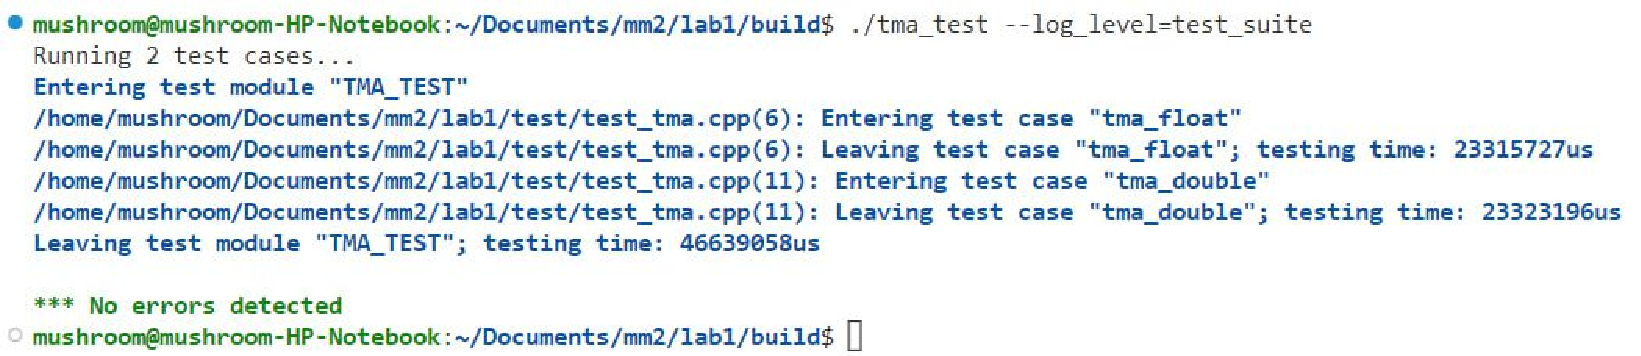
\includegraphics[width=\textwidth]{img/test.pdf}
\end{center}

\subsubsection{Интегро-интерполяционный метод}

Выполним нашу программу на ряде входных параметров

\begin{table}[H]
  \centering
  \begin{tabular}{ c | *{8}c }
    \toprule
    Номер теста & k & q & u & f & $\nu_1 $ & $\nu_2 $ & $R_L$ & $R_R$\\
    \midrule
    1 & r & 1 & 2r + 3 & 2r - 1 & -2 & 4 & 1 & 2 \\
    \midrule
    2 & $r^2$ & 1 & $2r^2 + 3$ & $-14r^2 + 3$ & -4 & 32 & 1 & 2 \\
    \midrule
    3 & $r^3$ & 1 & $2r^3 + 3$ & $-36r^4 + 2r^3 + 3$ & -6 & 192 & 1 & 2 \\
    \bottomrule
  \end{tabular}
\end{table}

После запуска программы мы получаем следующие результаты:
  \begin{table}[H]
    \centering
    \begin{tabular}{c | c | c}
      \toprule
      N & $ \left\lVert \varepsilon \right\rVert  $, одинарная точность & $ \left\lVert \varepsilon \right\rVert  $, двойная точность \\
      \midrule
      8 & 2.45905e-03 & 2.46952e-03\\
      16 & 6.10828e-04 & 6.19519e-04\\
      32 & 1.39713e-04 & 1.55015e-04\\
      64 & 6.91414e-05 & 3.87621e-05\\
      128 & 6.19888e-05 & 9.69106e-06\\
      256 & 2.66743e-03 & 2.42279e-06\\
      512 & 9.03511e-03 & 6.05706e-07\\
      1024 & 9.06944e-03 & 1.51435e-07\\
      2048 & 4.98871e-01 & 3.78822e-08\\
      \bottomrule
    \end{tabular}
    \caption{Погрешность теста №1}
  \end{table}

  \begin{table}[H]
    \centering
    \begin{tabular}{c | c | c}
      \toprule
      N & $ \left\lVert \varepsilon \right\rVert  $, одинарная точность & $ \left\lVert \varepsilon \right\rVert  $, двойная точность \\
      \midrule
      8 & 1.49273e-01 & 1.49265e-01\\
      16 & 3.73564e-02 & 3.73383e-02\\
      32 & 9.32503e-03 & 9.33596e-03\\
      64 & 1.68228e-03 & 2.33408e-03\\
      128 & 1.65176e-03 & 5.83525e-04\\
      256 & 1.83487e-03 & 1.45882e-04\\
      512 & 2.59638e-02 & 3.64704e-05\\
      1024 & 7.11317e-01 & 9.11763e-06\\
      2048 & 5.93484 & 2.27931e-06\\
      \bottomrule
    \end{tabular}
    \caption{Погрешность теста №2}
  \end{table}

  \begin{table}[H]
    \centering
    \begin{tabular}{c | c | c}
      \toprule
      N & $ \left\lVert \varepsilon \right\rVert  $, одинарная точность & $ \left\lVert \varepsilon \right\rVert  $, двойная точность \\
      \midrule
      8 & 2.52285 & 2.52289\\
      16 & 6.31502e-01 & 6.31225e-01\\
      32 & 1.5601e-01 & 1.57838e-01\\
      64 & 4.27036e-02 & 3.94614e-02\\
      128 & 1.83411e-02 & 9.86546e-03\\
      256 & 7.73621e-03 & 2.46637e-03\\
      512 & 2.19547e-01 & 6.16594e-04\\
      1024 & 1.32325 & 1.54148e-04\\
      2048 & 17.763 & 3.85369e-05\\
      \bottomrule
    \end{tabular}
    \caption{Погрешность теста №3}
  \end{table}

  Добавим еще один тест
  \begin{align*}
    k &= \frac{\ln(r)}{r} + 2 \quad q = \cos(r) \quad u = \sin(r) \\
    r &\in [\frac{\pi}{6}; \frac{\pi}{3} ]
  \end{align*}

  Находим значение $f$ как:
  \[
    -\left[ \frac{1}{r} \frac{d}{dr} \left(r \cdot (\frac{\ln(r)}{r} + 2 ) \cdot \frac{d \sin(r)}{dr} \right)\ -\ \cos(r) \cdot \sin(r) \right] = f(r),
  \]

  Получаем:
  \[
    f(r) = -\frac{(1+2r) \cos(r) - r \sin(r) (\ln(r) + 2r)}{r^2} + \cos(r)\sin(r)
  \]

  Находим значения $ \nu_1 $ и $ \nu_2 $:
  \begin{align*}
		& (\frac{\ln(r)}{r} +2) \left. \frac{d\sin(r)}{dr}\right\vert_{r = \frac{\pi}{6}} = -\nu _1
		&-(\frac{\ln(r)}{r} +2) \left. \frac{d\sin(r)}{dr}\right\vert_{r = \frac{\pi}{3}} = -\nu_2 \\
    & \nu_1 = -\frac{3 \ln(\frac{\pi}{6}) \sqrt{3} + \pi \sqrt{3}}{\pi} \\
    &\nu_2 = \frac{3\ln(\frac{\pi}{3}) + 2\pi}{2 \pi}
  \end{align*}
  \begin{table}[H]
    \centering
    \begin{tabular}{c | c | c}
      \toprule
      N & $ \left\lVert \varepsilon \right\rVert  $, одинарная точность & $ \left\lVert \varepsilon \right\rVert  $, двойная точность \\
      \midrule
      8 & 2.18486e-3 & 2.18486e-3\\
      16 & 5.07295e-4 & 5.50816e-4\\
      32 & 2.44796e-4 & 1.38007e-4\\
      64 & 1.33216e-4 & 3.45209e-05\\
      128 & 6.25908e-4 & 8.63144e-06\\
      256 & 1.61629e-2 & 2.15794e-06\\
      512 & 8.05649e-2 & 5.39484e-07\\
      1024 & 2.45799e-1 & 1.34881e-07\\
      2048 & 6.22395 & 3.36463e-08\\
      \bottomrule
    \end{tabular}
    \caption{Погрешность теста №4}
  \end{table}

На данных тестах можно проследить зависимость погрешности от числа разбиений, которую мы выявили в предыдущей главе, что при увеличении шага
в 2 раза погрешность должна уменьшаться примерно в 4 раза. Также можно проследить что есть число разбиений при котором погрешность минимальна.
При дальнейшем увеличении числа разбиений погрешность увеличивается (данное явление можно заметить на тестах одинарной точности).
	\newpage

	\section{Заключение}
	\subsection{Вывод}
	Задание выполнено в полном объеме.
	Был написан написан метод приближенного вычисления краевой задачи и метод прогонки, а также написаны тесты к ним.
	Была оценена погрешность и выявлена зависимость погрешности от числа разбиения.
	\newpage
	\subsection{Код}
	\inputminted{c++}{../lab1/src/main.cpp}
	\inputminted{c++}{../lab1/src/data_table.hpp}
	\inputminted{c++}{../lab1/include/tma.hpp}
	\inputminted{c++}{../lab1/include/balance.hpp}
	\inputminted{c++}{../lab1/include/utils.hpp}
	\inputminted{c++}{../lab1/include/utils/balance_utils.hpp}
	\inputminted{c++}{../lab1/include/utils/data.hpp}
	\inputminted{c++}{../lab1/include/utils/grid.hpp}
	\inputminted{c++}{../lab1/test/test_tma.cpp}
	\inputminted{c++}{../lab1/test/test_utils.hpp}
\end{document}